% Chapter 1

\chapter[Motivation and Background]
{Motivation and Background} % Main chapter title

\label{Chapter1} % For referencing the chapter elsewhere, use \ref{Chapter1} 

%----------------------------------------------------------------------------------------






% Define some commands to keep the formatting separated from the content 
\newcommand{\keyword}[1]{\textbf{#1}}
\newcommand{\tabhead}[1]{\textbf{#1}}
\newcommand{\code}[1]{\texttt{#1}}
\newcommand{\file}[1]{\texttt{\bfseries#1}}
\newcommand{\option}[1]{\texttt{\itshape#1}}

%----------------------------------------------------------------------------------------

\section[Quantum info processing and Qubit candidates]{Quantum info processing and Qubit candidates}

The bit is the basic unit of information in computing and digital communications. A bit can have one value, which can be 1 or 0, that represents the logical states in a 2-level logic system. In modern digital computers, these two states exits as low and high voltages in highly integrated circuits. Just like bit for classical computing, qubit is the basic unit of information in QIP, which encodes 1 and 0 into 2 distinguishable quantum states. As the qubits behaves in the manner of quantum mechanism, it gives rise to the phonomena of superposition and entanglement, which enables the processing of massive number of calculations. Previous difficult tasks in classical computing such as simulation of quantum systems or factoring of numbers will be finished quick and efficiently by quantum computers.

For the realisation of quantum computer,  the first priority is to find a fitting candidate as qubit. Five principles have been brought up for the candidates choosing by [Journal,name]:

1. A scalable physical system with well characterized qubits

2. The ability to initialize the state of qubits to a simple fiducial state

3. Long relevant decoherence times, much longer than gate operation time

4. A "universal" set of quantum gates

5. A qubit-specific measurement capability

Color centers are optically active impurities that are responsible for the colors in crystal that are transparent due to large band gap. Color centers are atom-like solid systems, with appropriate electronic structure and symmetry in crystal, they are the candidates for qubits. Additionally, it is practical to require a long enough coherent time for the operation regarding QIP.

Lots of research works has been done with NV$^{-}$, which has excellent spin properities at ambitent condition, it has also been proved that it is possible to execute an all optical access to its spin.[reference from all optical paper]. Yet due to the transform of symmetry during the excitation process, NV$^{-}$ has a big phonon side band following the ZPL. Moreover, the C3v symmetry leaves the color centre vulnerable towards the environment electric field, resulting in spectral diffusion, which is caused by the flipping of charging state. These disadvantages has reduced the generation rate of coherent photon generation rates and limit the development of NV-quantum networks[Lachlan paper].
%----------------------------------------------------------------------------------------

\section[Silicon vacancy as a Qubit candidate]{Silicon vacancy as a Qubit candidate}

SiV is considered as the next promising qubit candidate after NV. It has irresistibly excellent optical properties, and is also possible to achieve an all optical intiallizaiton, read out and coherent preparation.

SiV$^{-}$ has a D$_{3d}$ symmetry with the symmetry axis along the <111> crystal direction. The color center consists of a substitial Silicon atom and a carbon vacancy. Due to the size difference between Silicon atoms and carbon atoms, it is expected that the Silicon atom will sit between 2 lattice site instead of on a lattice site[Goss etal,  Gali and Maze, ]. The inversed symmetry offers SiV$^{-}$ extra shield from the environment small electric field.

Experimentally it is observed that the SiV$^{-}$ has outstanding optical properties, 70$\%$ of its fluorescence couples into a sharp ZPL of 1.68eV. At cryogenic temperature this ZPL can be resolved with a fine structure of 4 lines. These four lines are signed to the electronic transitions between the ground state and the first excited state of SiV$^{-}$. Theoretical calculation based on the group theory and ab initio method offers us a model of the SiV$^{-}$ electronic structure with a ground state of 2 folded degeneracy and even parity, a first excited state of 2 folded degeneracy of uneven parity and a second excited state of none degeneracy with even parity.[Goss etal] This calculation fits the observation as only the electronic transition between levels of different parity is allowed, due to the -1 parity of photons, thus only the 4 transitions between the first excited state and the ground state would be allowed, as signed to the 4 line structure of ZPL. Since this is a E to E transition, no dramatic symmetry change has been involved, less phonon would be involved in the relaxation, which fits the observation of the sharp ZPL with small phonon side band. 

Lachlan et al showed the probility to read out and coherently prepare electronic spin in individual SiV$^{-}$ centers via resonance excitation. The SiV$^{-}$ was first initialized by resonantly pumping the spin-flipping transition D1 that is weakly allowed due to the off axis residue of the magnetic field, this is done with applying a laser pulse that resonant to transition D1. After a dark interval the spin state was read out using a laser pulse on the cycling transition D2. The leading edge peak from D2 pulse will decrease with the increase of dark interval approaching an minimum. From which the spin relaxation time T1 has be calculated as 2.4 $\pm$ 0.2ms. With the similar pulse measurement, the orbital T1 has been measured as 38 $\pm$ 1ns. The fact that the orbital T1 is much shorter that spin T1 indicates that the orbital relaxation is highly spin conserving, as the electron phonon interaction should be.  The temperature dependency measurement reveals that the orbital rate increase linear with the temperature until 22K, which indicates a single-phonon mechanism of orbital relaxation.[Lachlan et al,and 30-32 from the paper]

Further CPT was carried out by tuning the pump laser to transition D2 while scanning across the transition D1 using the probe laser. The spin coherent time was then measured to be 35 $\pm$ 3ns. This short coherence time is likely to be connected to the dephasing caused by the rapid orbital relaxation.

Practically, as mention before, a qubit candidate ideally need to have long enough coherent time for the implementation of operation and read out, in this sense, the short coherent time of SiV$^{-}$ drawed it back from being an competitive qubit candidate. 

Several ideas of acquiring longer coherence time has been taken into consideration. While most of them can be classified into two main approaches: avoid orbital relaxation caused electron spin dephasing by accessing the orbital spin in Si$^{29}$ or eliminate the single phonon that has been involved in the orbital relaxation.

\begin{figure}[h]
\centering
\includegraphics[width=1\linewidth]{Figures/pic/WP_20160921_20_40_25_Pro_LI}
\caption{}
\label{fig:wp20160921204025proli}
\end{figure}

\begin{figure}[h]
\centering
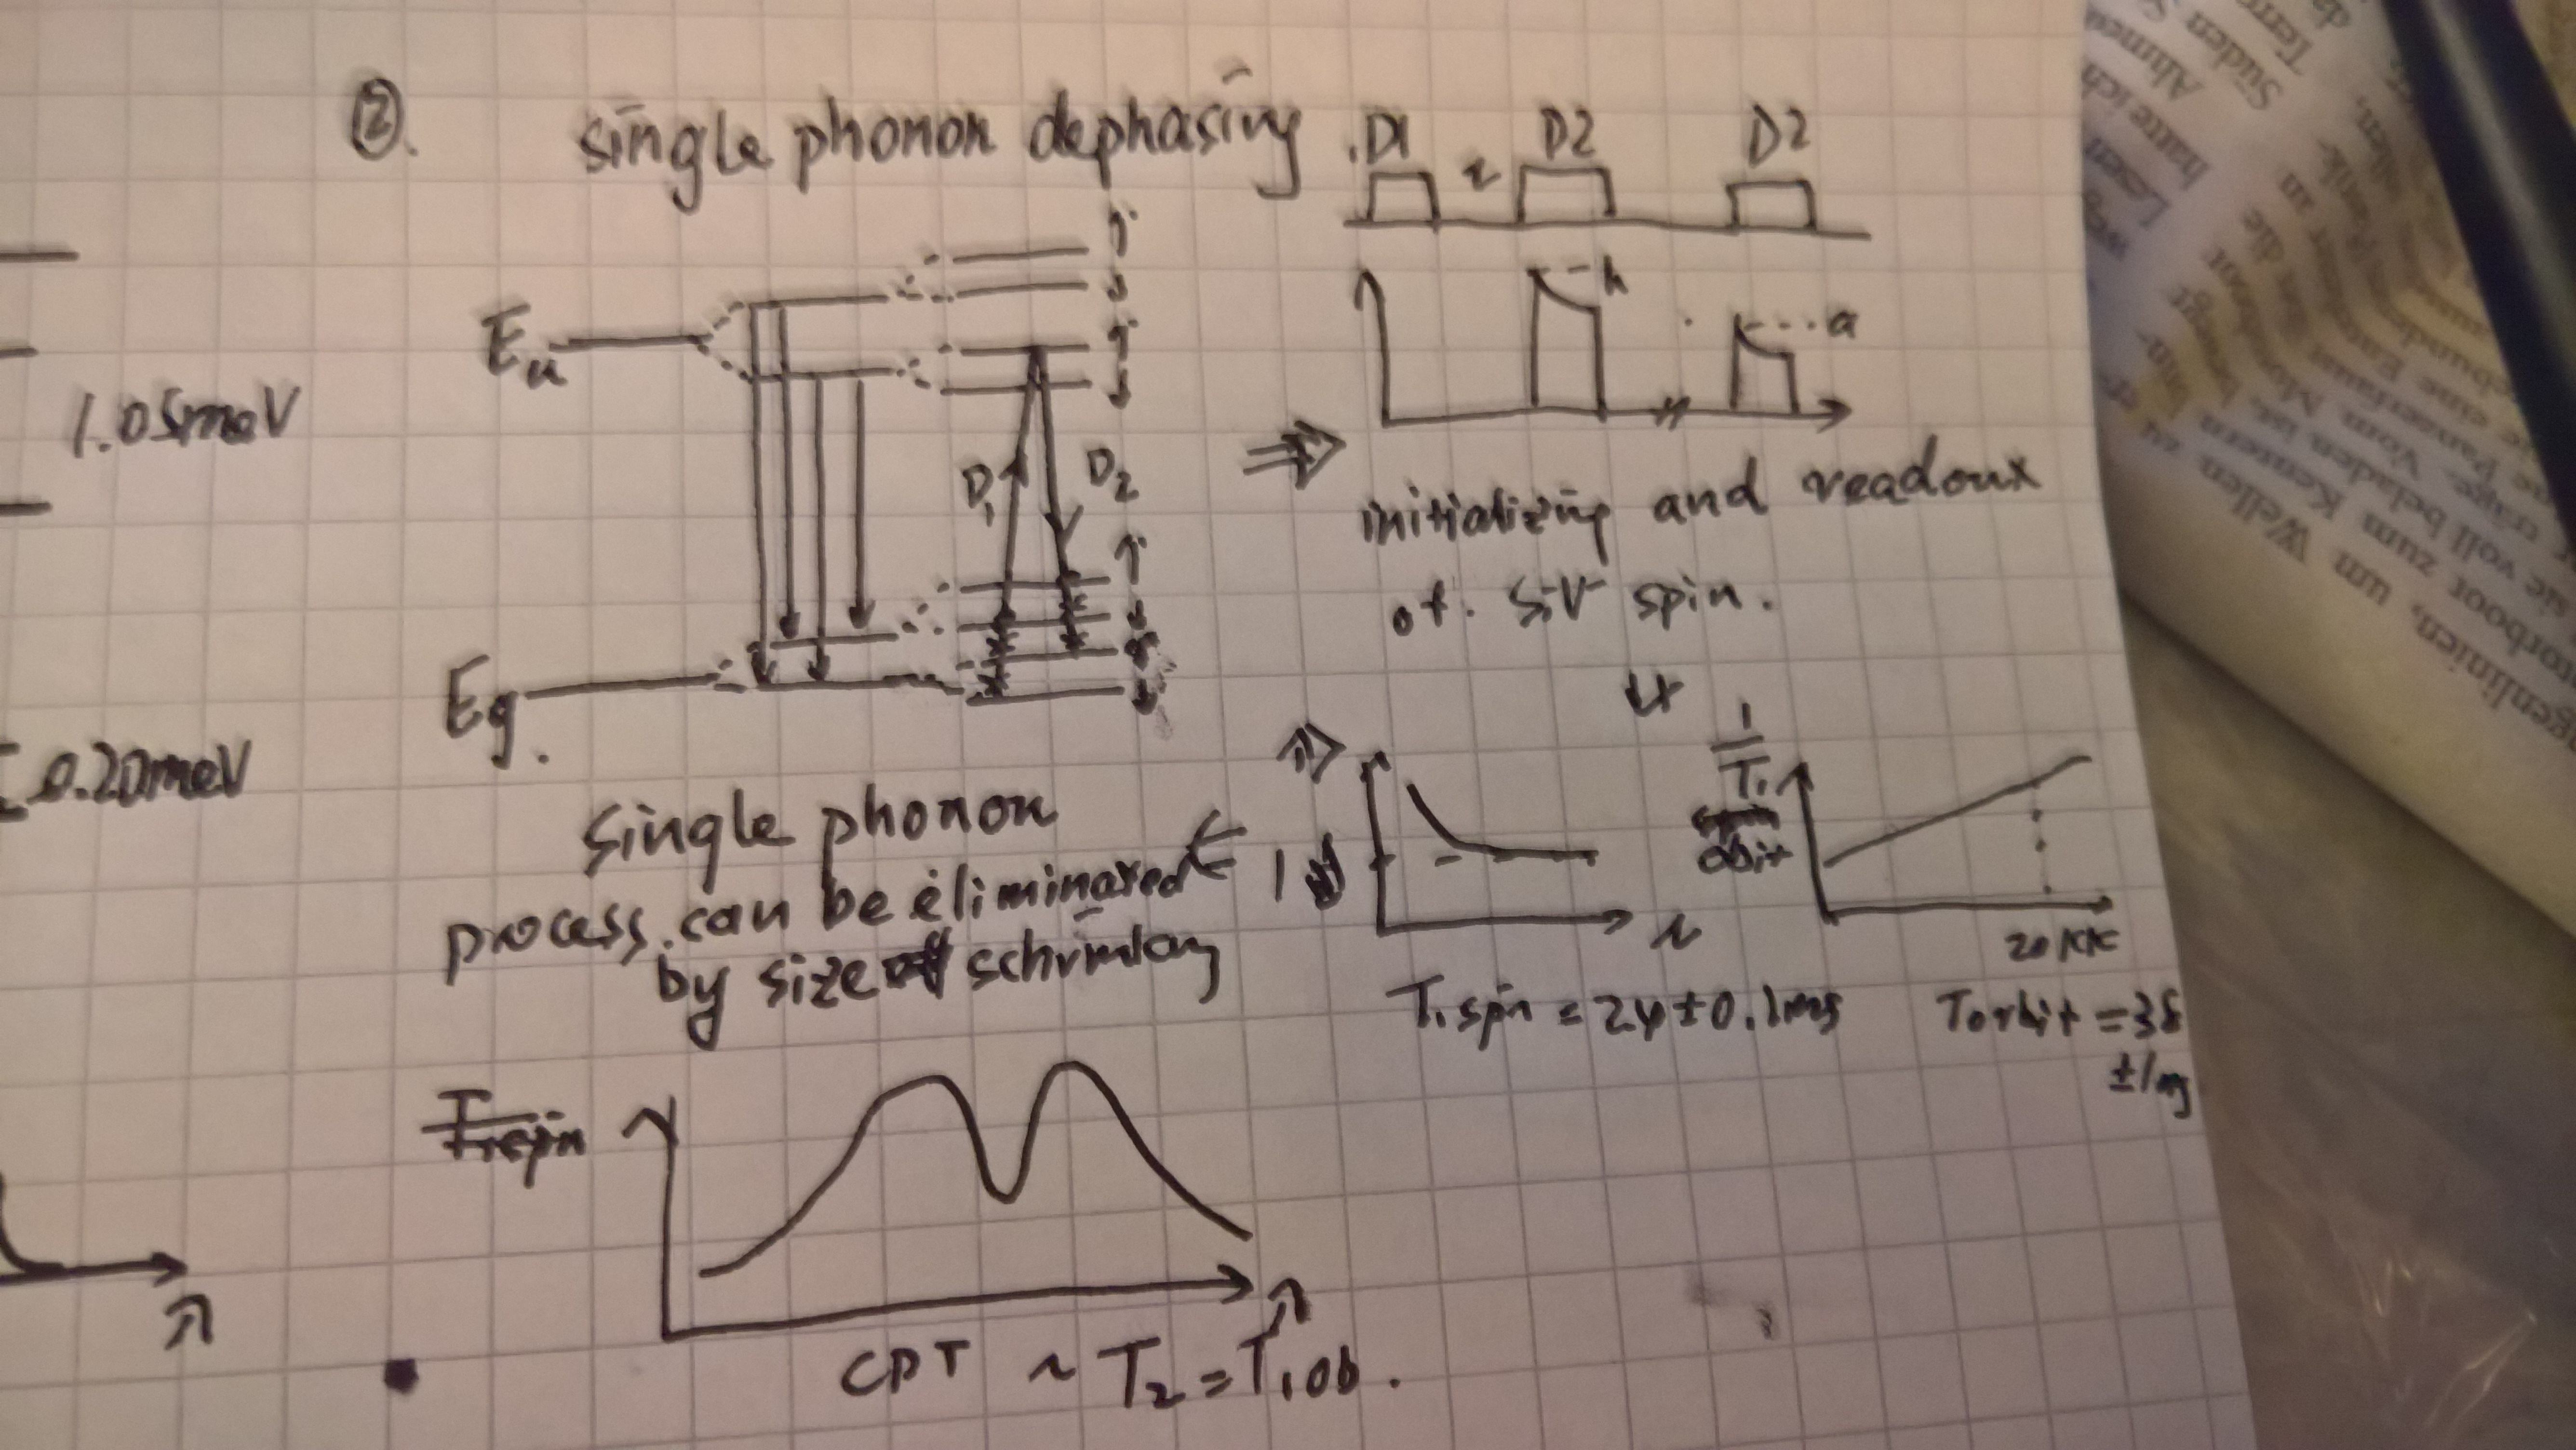
\includegraphics[width=1\linewidth]{Figures/pic/WP_20160921_20_40_32_Pro_LI}
\caption{}
\label{fig:wp20160921204032proli}
\end{figure}

%----------------------------------------------------------------------------------------

\section[Silicon vacancies in nanodiamonds]{Silicon vacancies in nanodiamonds}
\begin{figure}[h]
\centering
\includegraphics[width=1\linewidth]{Figures/pic/WP_20160921_20_40_48_Pro_LI}
\caption{}
\label{fig:wp20160921204048proli}
\end{figure}
As mentioned, one vital problem to solve if we want to use SiV$^{-}$ as a qubit is that, the coherent time has been limited by the rapid orbital relaxation. And this is caused by the transition between the degeneracies of ground state which was driven by a single phonon. The elimination of such phonon is an direct approach towards the solution.

Spontaneous emission is inhibited if the cavity has characteristic dimensions which are small compared to the radiation wavelength [Daniel Kleppner1981]. As in our case to eliminate the emission of phonon that couples into the splitting of ground state in SiV$^{-}$ 47 GHz, nanodiamond of the size that is smaller than the half wavelength of this transition phonon wavelength (around 125nm) is desired. 

Currently 3 major techniques are employed in the field of nanodiamond fabrication: denotation, CVD, and HPHT, while the exotic atoms can be mixed in the beginning or implanted via ion implantation. While the denotation method produced highly defective diamonds and ion implantation introduces inner strain, for the SiV containing nanodiamonds, HPHT method and CVD method are the top choices.

The principle of CVD method is to disintegrate the CVD fabricated diamond film, while the HPHT method initialize an phase transition of carbon at high temperature and high pressure. Previously, comparison between the PL spectra of silicon doped polycrystalline diamond films obtained by the CVD method and diamond single crystals grown at a pressure of 6 GPa from a nickel melt at 1500$^{o}C$ has been carried out, and demonstrates that the HPHT diamonds carries narrower SiV$^{-}$ ZPL lines than CVD fabricated ones[C. D. Clark 1995]. As in the department of nanodiamonds, the narrowest SiV$^{-}$ ZPL that has been measued by far, which has a corrected width of 206MHz, that is almost of the excitation state life time limit, is also from the HPHT method fabricated nanodiamond.

%--------------------------------------------------------------------------------------

\section[Motivation of the thesis, unsolved problem]{Motivation of the thesis}
\FloatBarrier
\begin{figure}[h]
	\centering
	\includegraphics[width=1\linewidth]{Figures/pic/WP_20160921_20_40_42_Pro_LI}
	\caption{}
	\label{fig:wp20160921204042proli}
\end{figure}
\FloatBarrier
The motivation of looking into SiV$^{-}$ in nanodiamonds is to acquire longer coherent time by eliminating the phonon that is responsible for the transition between the fine splitting of the ground state. Yet the obstacle on our way of justifying this approach is that, the optical properties of SiV$^{-}$ in nanodiamonds are not as outstanding as it is in bulk diamond. Blinking and spectral diffusion, especially spectral diffusion has stopped us from further life time measurement. 

The mechanism behind the spectral diffusion is yet not clear, our first guess is to connect the enhancement of spectral diffusion in nanodiamonds with the surface condition, due to the high surface to volume ratio of nanodiamonds.

Our target of this thesis is to improve the optical properties of nanodiamonds, more specifically, to suppress the spectral diffusion via methods of surface treatment, enabling further measurements including but not limited at orbital/spin T1 and coherent population trapping, and finally to test out the possibility of acquiring a longer coherent time via the elimination of the single phonon process.
  
In the synthesis procedure of HPHT nanodiamonds, due to the surface absorption of nitrogen on ingredients, NV can be introduced. N atoms act as a n-type dopant, an electron donor in the diamonds. Due to the different dopant density on the surface and in crystal, to match chemical potentials at the surface and in the bulk, charge builds up on the surface depleting the donor charges a depth into the bulk and bending the bands accordingly. 

\begin{figure}[h]
\centering
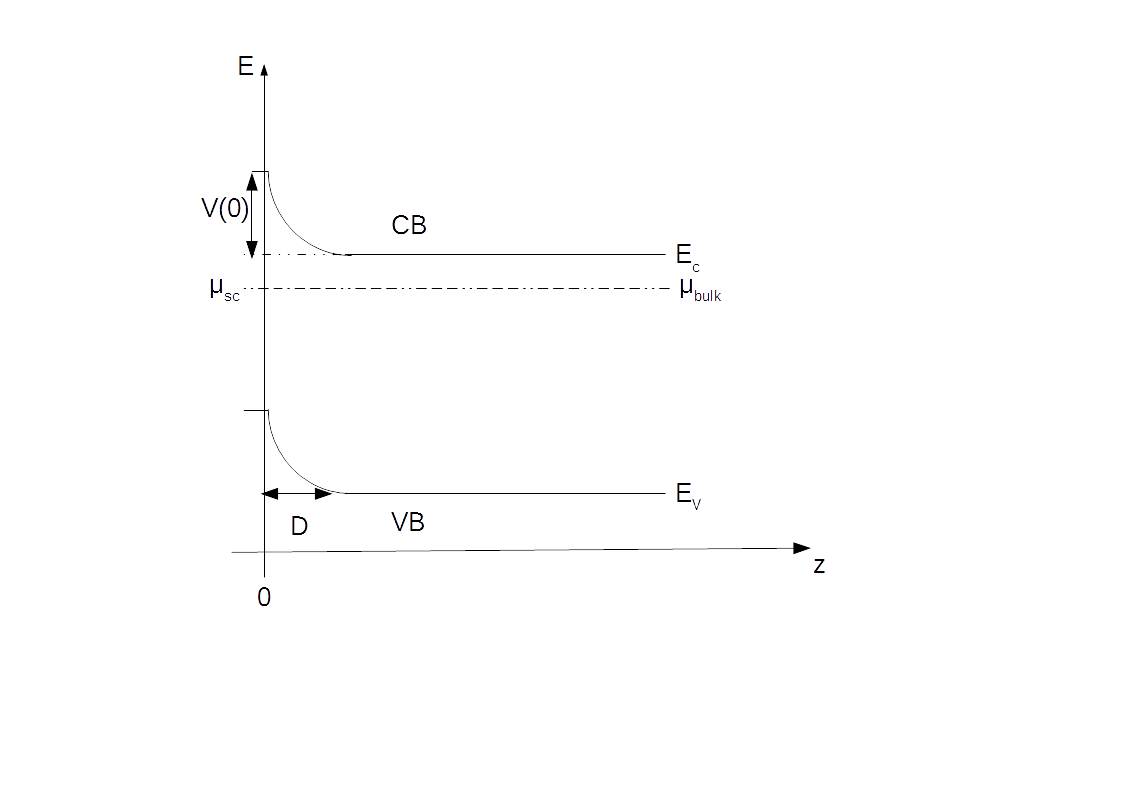
\includegraphics[width=0.7\linewidth]{Figures/pic/bandbending}
\caption{A sketch describing the band-bending of n-doped diamond. Since the chemical potential of the surface and the doped bulk area need to match up with each other, a depletion layer is formed, the bands (CB: conducting band, VB:valence band) bends towards up near the surface.  }
\label{fig:bandbending}
\end{figure}

The width of this depletion layer can be calculated with the equation

$D = \sqrt{\frac{2\psi V(0)}{qN_{D}}}$, 

where $\psi$ is the dielectric constant, V(0) is the band bending and $N_{D}$ is the concentration of dopant. As in our case, the concentration of Nitrogen is not clear but expected to be low, thus resulting in broader depletion layer. With a typical moderate dopant concentration of 10$^{-16}/cm^{3}$, the width of depletion layer is calculated to be 80nm[Diederich,1998]. As mentioned before, to inhibit the generation of 47 GHz phonons, the diameter of the diamonds need to be smaller than 125nm, and there is a high chance that SiV in nanodiamonds will lie in side or close to the band bending area, which may be the cause of spectral diffusions.

It is expected to flatten the band bending by inhibit the surface charge accumulation. In this thesis, 2 methods are applied. 

First is to remove the graphitic defect by aerobic oxidation. Aerobic oxidation is a good method for surface purification and initialization. Research on denotation diamonds shows that, with the temperature between 375$^{o}C$ to 450$^{o}C$,the removal of $Sp^{2}$[Osswald,2006]. After 2h of aerobic oxidation at 575$^{o}C$, the surface structure of HPHT NDs is very similar to bulk single crystals where hydroxyl and possibly ethers are the dominant functional groups[Wolcott 2014]. Aerobic oxidation with elevated temperature can cause the size reduction of nanodiamonds. It has been reported that the average height reduction rate of individual crystals was 10$\pm$1nm/h at 600$^{o}C$, 4$\pm$1nm/h at 550$^{o}C$ and less than 1nm/h at 500$^{o}C$ from aerobic oxidation. Since graphitic defects on the surface of diamond are possible electron trap candidate[ J. Ristein, Diamond Relat. Mater. 9, 1129 (2000). ], it is possible to lower the surface charge via aerobic oxidation.

The second method is to achieve negative electron affinity via Hydrogen termination, due to the electrostatic effect of the dipole moment p of the heteropolar $C^{\text{-}} H^{+}$ bonds. As most of the reducing agents would rather form different types of hydroxyl groups on the surface than replace the surface groups with C-H bond, only the direct reaction with elemental hydrogen enables the formation of C-H bond as surface termination. Hydrogen plasma has been applied to bulk diamond and diamond thin film as a method to achieve full coverage of hydrogen termination as well as to nanodiamond powers[Yeap Langmuir 2009].
